\paragraph{1.2.4. GAT Layers (Tầng GAT)}
\indent\indent Đây là thành phần cốt lõi thực hiện quá trình truyền tin (Message Passing) để cập nhật đặc trưng nút, với kiến trúc được minh hoạ như \textbf{Hình \ref{fig:KTGATLayers}}.

\begin{figure}[H]
    \centering
    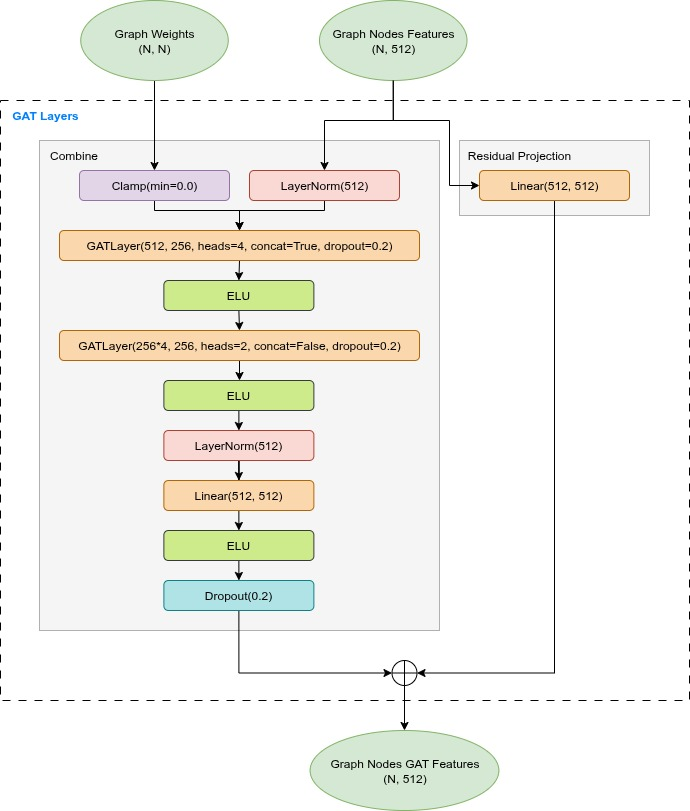
\includegraphics[width=0.8\linewidth]{images/part-02/chap-02/sec-01/GATLayers.jpg}
    \vspace{0.3cm}
    \caption{Kiến trúc của GAT Layers với cơ chế Weighted Message Passing}
    \label{fig:KTGATLayers}
\end{figure}

Mô hình áp dụng biến thể Weighted GAT kết hợp với Dynamic Attention. Khác với GAT truyền thống chỉ dựa vào đặc trưng nút và ma trận kề để tính hệ số attention, thì mô hình trong đề tài này tích hợp trực tiếp trọng số cạnh học được ($GW_{ij}$) vào quá trình tính toán, với công thức cụ thể như sau:
\[
    \alpha_{ij} = \text{softmax}(\text{LeakyReLU}(\vec{a}^T [W\vec{h}_i \| W\vec{h}_j]) \cdot {GW}_{ij})
\]
\indent Trong đó $GW_{ij}$ là ma trận trọng số cạnh của đồ thị từ tầng trước đã qua hàm \texttt{Clamp(min=0.0)} để loại bỏ giá trị âm. Cơ chế này giúp khắc phục hạn chế "Static Attention", cho phép mô hình kiểm soát luồng thông tin linh hoạt hơn: các cạnh có trọng số lớn sẽ khuếch đại tín hiệu, ngược lại các cạnh yếu sẽ bị chặn lại. Hàm kích hoạt phi tuyến ELU (Exponential Linear Unit) được sử dụng sau mỗi lớp GAT nhằm hỗ trợ việc học các biểu diễn của vector tốt hơn và tăng tốc độ hội tụ so với ReLU thông thường \cite{clevert2016fastaccuratedeepnetwork}.\vspace{0.3cm}

Ngoài ra, tầng này cũng được áp dụng thêm kỹ thuật Pre-LayerNorm (chuẩn hóa trước khi đưa vào layer) để ổn định gradient khi huấn luyện mô hình sâu, tránh hiện tượng bùng nổ hoặc biến mất gradient thường gặp trong các mạng GNN nhiều lớp \cite{xiong2020layernormalizationtransformerarchitecture}. Tương tự các tầng trước, cơ chế Residual Connection vẫn được duy trì để bảo toàn thông tin gốc qua các phép biến đổi phức tạp.